\begin{figure}[!htb]
\begin{center}
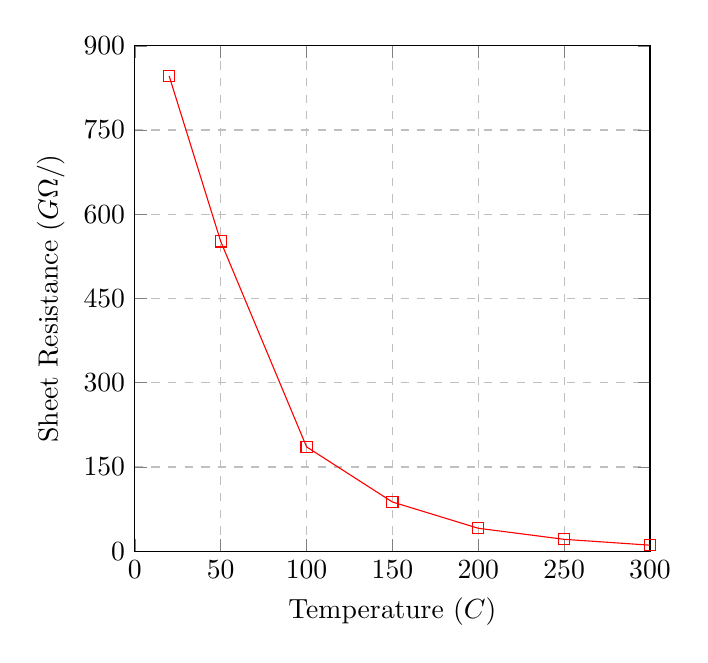
\begin{tikzpicture}

\begin{axis}[
    %title={Temperature dependence of CuSO$_4\cdot$5H$_2$O solubility},
    xlabel={Temperature ($\degree C$)},
    ylabel={Sheet Resistance ($G\Omega/\msquare$)},
    height=8cm,
    width=0.67\textwidth,
    xmin=0, xmax=300,
    ymin=0, ymax=900,
    xtick={0, 50, 100, 150, 200, 250, 300},
    ytick={0, 150, 300, 450, 600, 750, 900},
    legend pos=north east,
    xmajorgrids=true,
    ymajorgrids=true,
    grid style=dashed,
]

\addplot[color=red, mark=square]
  coordinates {
    (20, 846.0)
    (50, 551.6)
    (100, 185.8)
    (150, 87.62)
    (200, 40.84)
    (250, 21.16)
    (300, 10.72)
};

\end{axis}
\end{tikzpicture}

\caption{Plot of Sheet Resistance vs Temperature on Substrate A}
\label{fig:results:sheet_against_temp}
\end{center}
\end{figure}
